\documentclass[preprint,12pt]{elsarticle}

\ifdefined\synctex
  \synctex=1
\fi

\usepackage{amssymb}
\usepackage{amsmath}
\usepackage[a4paper,margin=1in]{geometry}
\usepackage{graphicx}
\usepackage{booktabs}
\usepackage{subcaption}
\usepackage{caption}
\usepackage{float}
\usepackage{algorithm}
\usepackage{algpseudocode}
\usepackage{multirow}
\usepackage{array}
\usepackage{enumitem}
\usepackage{needspace}
\usepackage[hidelinks]{hyperref}
\hypersetup{pdfauthor={},pdfsubject={},pdfkeywords={}}
\usepackage{fontspec}
\usepackage{xeCJK}
\setCJKmainfont{SimSun}

\graphicspath{{./figures/}}
\journal{Engineering Applications of Artificial Intelligence}

\setcounter{topnumber}{3}
\setcounter{bottomnumber}{2}
\setcounter{totalnumber}{5}
\renewcommand{\topfraction}{0.9}
\renewcommand{\bottomfraction}{0.8}
\renewcommand{\textfraction}{0.07}
\renewcommand{\floatpagefraction}{0.8}

\renewcommand{\algorithmicrequire}{\textbf{Require:}}
\renewcommand{\algorithmicensure}{\textbf{Ensure:}}

\captionsetup[figure]{name=Fig.}
\captionsetup[table]{name=Tab.}

\newcommand{\figref}[1]{Fig.\nobreakspace\ref{#1}}
\newcommand{\tabref}[1]{Tab.\nobreakspace\ref{#1}}

\begin{document}

\begin{frontmatter}

\title{Reinforcement Learning-Based Computer Numerical Control Motion Planning with Adaptive Preview and Jerk-Constrained Action Projection}

\begin{abstract}
Computer numerical control (CNC) motion planning must convert CAM-generated tool paths into executable interpolation trajectories that satisfy contour tolerance and kinematic limits. Conventional pipelines usually smooth the path first and then plan the feedrate. Once the path is fixed, however, feedrate planning can only adjust speed along a prescribed curve and cannot use the tolerance band to reshape corner or curvature-transition motion. This separation weakens the coupling between geometric smoothing and dynamic feasibility. To address this issue, this paper proposes J-NNC, a closed-loop reinforcement learning framework for tolerance-band CNC motion planning. A Proximal Policy Optimization (PPO) policy predicts steering, feedrate, and preview-distance actions from structured tracking, kinematic, corner, and forward-geometry states. A kinematic constraint module (KCM) then projects the raw policy outputs into executable commands satisfying linear and angular velocity, acceleration, and jerk limits. Experiments on square, circular, and butterfly-shaped paths show that J-NNC completes all cases with full path progress and eliminates the linear-jerk violations observed in the neural network controller (NNC) baseline and the no-KCM ablation.
\end{abstract}

\begin{keyword}
computer numerical control \sep reinforcement learning \sep learnable preview distance \sep jerk-constrained action projection
\end{keyword}

\end{frontmatter}

\section{Introduction}
\label{sec:introduction}
Conventional CNC motion planning usually follows a serial pipeline: the tool path is smoothed first, and feedrate planning is then carried out along the smoothed path~\cite{Sun2022,Yan2023}. This procedure improves the geometric continuity of CAM-generated tool paths. Once the smoothed trajectory is fixed, however, the feedrate planner can mainly adjust the motion speed along that trajectory~\cite{Erkorkmaz2001,Lee2011}. It has little room to reuse the spatial freedom inside the contour-tolerance band, especially in corner regions and curvature-transition regions~\cite{Sencer2015,Tajima2016}. For this reason, geometric smoothness, feedrate efficiency, and kinematic feasibility under velocity, acceleration, and jerk limits are difficult to optimize together in high-precision, high-speed machining~\cite{Sun2022,Zhang2021}.

In practice, this serial pipeline is built mainly from local smoothing, global smoothing, and feedrate scheduling. Local smoothing constructs transition curves between adjacent blocks. It is well suited to real-time interpolation because the computation is local and the contour error can be bounded explicitly~\cite{Hu2024}. Higher-order B\'ezier, B-spline, and curvature-smooth transitions can further improve acceleration or jerk continuity around corners~\cite{Fan2015,Zhang2018}. Dense short segments and consecutive corners, however, often leave only a limited transition length~\cite{Li2020}. Global smoothing reconstructs several segments over a larger domain and improves continuity for dense short-block paths~\cite{Song2021}. Under strict contour-error constraints, however, computational cost, iterative fitting, local feature preservation, and real-time implementation remain difficult~\cite{Yang2015}. Feedrate scheduling imposes velocity, acceleration, and jerk bounds along a selected path, but it usually starts from a predetermined geometric trajectory~\cite{Zhang2021}. NURBS and S-shaped schemes improve feasibility under chord-error and axial-drive constraints~\cite{Wu2022}. Look-ahead interpolation uses upcoming path information to regulate feedrate over short-line or spline tool paths~\cite{Tsai2010,Song2020}. These studies provide the main technical basis of the conventional serial CNC motion-planning pipeline.

Although this line of work has made substantial progress, the serial decomposition still separates geometry selection from timing regulation, even though these two decisions are physically coupled during interpolation. Local and global smoothing first determine the geometric curve used inside the contour-tolerance band, including the corner-transition shape and the curvature distribution. Feedrate scheduling then assigns a speed profile to the selected curve. The later stage can reduce or increase the feedrate, but it has limited ability to change how the tolerance band is used geometrically. This separation is especially restrictive when short segments, consecutive corners, and rapidly varying curvature appear in the same CAM path~\cite{Li2020,Zhao2013}. A conservative smoothing result may cause unnecessary deceleration, while an aggressive transition may still require speed reduction to satisfy acceleration or jerk limits~\cite{Sencer2015,Tajima2016}. Thus, a fixed serial procedure leaves limited room to balance the geometric use of the tolerance band with jerk-limited executable motion~\cite{Sun2022,Zhang2021}.

To address the limitations of the conventional serial pipeline, one-step methods aim to perform trajectory smoothing and feedrate planning within a unified planning process. Direct axis-velocity blending and integrated acceleration/deceleration interpolation plan axis motion near corners under real-time constraints~\cite{Tajima2016,Tsai2016}. Minimum-time cornering and high-speed cornering with vibration suppression optimize corner traversal under contour-error and actuator limits~\cite{Sencer2015,Duan2016}. Driving-force-constrained smoothing brings drive capability into corner planning, and quadratic B-spline fitting combines tool-path construction with optimal velocity interpolation under bounded error~\cite{Yang2015,LiDriving2017}. Integrated smoothing methods for line--arc and five-axis paths further handle transition overlap and feedrate fluctuation within unified smoothing procedures~\cite{Li2023,Sun2024}. In a closely related direction, Li et al. proposed neural-network numerical control (NNC), which treats CNC trajectory smoothing as a closed-loop action-decision problem and directly generates angle-change and step-length-change commands at each interpolation cycle~\cite{Li2020}. NNC shows that trajectory generation inside the tolerance band can be learned as an online decision process, with higher machining efficiency than local smoothing and higher contour accuracy than global smoothing~\cite{Li2020}.

These one-step methods strengthen the connection between path geometry and speed behavior, but several issues remain for tolerance-band CNC motion planning. Many optimization-based methods rely on predefined transition forms, local corner models, nonlinear constraints, or iterative computation. Their performance can therefore be sensitive to segment length, corner distribution, and local geometry variation~\cite{Yang2015,Li2023}. In NNC, the neural-network action is converted directly into an interpolation position or a servo command. If velocity, acceleration, and jerk constraints are not handled explicitly, or if no projection is applied at the execution layer, the generated command may violate the kinematic limits of the machine tool~\cite{Li2020}. In addition, the reward design mainly focuses on contour error, while path progress, direction consistency, motion smoothness, and stage-dependent behavior near corners receive less attention~\cite{Li2020}. These limitations make it difficult for one-step planning to use the tolerance band effectively, maintain path advancement, and guarantee executable interpolation under jerk constraints at the same time.

This paper addresses these issues by proposing J-NNC (Jerk-constrained Neural Numerical Controller), a reinforcement learning-based CNC motion-planning framework with jerk-constrained action projection and adaptive preview. The framework formulates mixed-tool-path motion planning as a constrained one-step decision problem within the contour-tolerance band. A kinematic constraint module (KCM) is inserted between the learned policy and the execution layer. It maps unconstrained steering and feedrate intentions to interpolation control variables that satisfy velocity, acceleration, and jerk constraints. The policy is trained using PPO~\cite{Schulman2017PPO} and outputs steering, feedrate, and preview-distance adjustment actions in a closed loop. The state representation includes tracking, kinematic, corner, and multi-scale forward-geometric information, and the reward accounts for path progress, contour error, direction consistency, and motion smoothness. \figref{fig:comparison_arch} compares conventional serial motion planning with the closed-loop J-NNC motion-planning framework.

\begin{figure}[htbp]
\centering
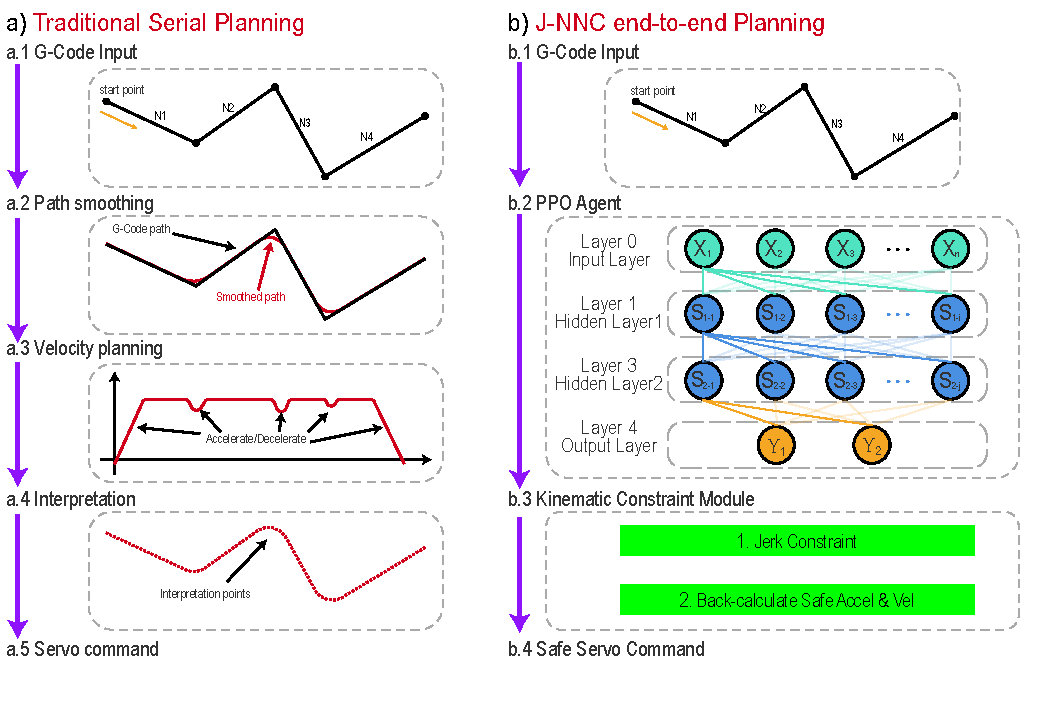
\includegraphics[width=0.9\linewidth]{Figure_1.pdf}
\caption{Comparison of conventional serial motion planning and the J-NNC motion-planning framework. J-NNC denotes the Jerk-constrained Neural Numerical Controller, a neural-network-based CNC motion planner with jerk-constrained action projection.}
\label{fig:comparison_arch}
\end{figure}

The main contributions are as follows:
\begin{enumerate}
\item[(1)] A KCM is developed to project raw steering and feedrate outputs into executable commands while satisfying velocity, acceleration, and jerk limits for both linear and angular motion.
\item[(2)] A tolerance-band one-step decision formulation with adaptive preview is proposed to jointly learn trajectory shaping and feedrate regulation from structured geometric and kinematic states.
\item[(3)] Experiments on square, circular, and butterfly-shaped paths show that J-NNC completes the full path and removes the linear-jerk-limit violations observed in the NNC baseline and the no-KCM ablation.
\end{enumerate}

The remainder of this paper is organized as follows. Section 2 defines the problem and models the constraints. Section 3 presents the proposed method. Section 4 reports the experimental settings, comparative results, and ablation analysis. Section 5 concludes the paper.

\section{Problem Formulation}
\label{sec:problem_formulation}
This section defines the motion-planning problem considered in this study, together with the geometric and execution constraints used in the proposed method. These definitions provide the basis for the method described in the following sections.

\subsection{Tool Path and Geometric Feasible Region}
Consider a discrete sequence of cutter-location points generated by a CAM system,
\begin{equation}
P_{\mathrm{raw}}={p_1,p_2,\dots,p_N},
\end{equation}
where $p_i\in\mathbb{R}^2$ denotes a reference point in the interpolation plane. Let $\varepsilon$ denote the prescribed contour tolerance. The reference path is offset by $\varepsilon/2$ on both sides to define the geometric feasible region in which the policy may locally deviate from the reference path:
\begin{equation}
\Omega={x\mid d(x,P_{\mathrm{raw}})\leq \varepsilon/2},
\label{eq:feasible_region}
\end{equation}
where $d(x,P_{\mathrm{raw}})$ denotes the minimum distance from point $x$ to the reference path. This region allows local redistribution of the trajectory within the tolerance band, which helps smooth corner traversal while preserving contour accuracy.

\begin{figure}[htbp]
\centering
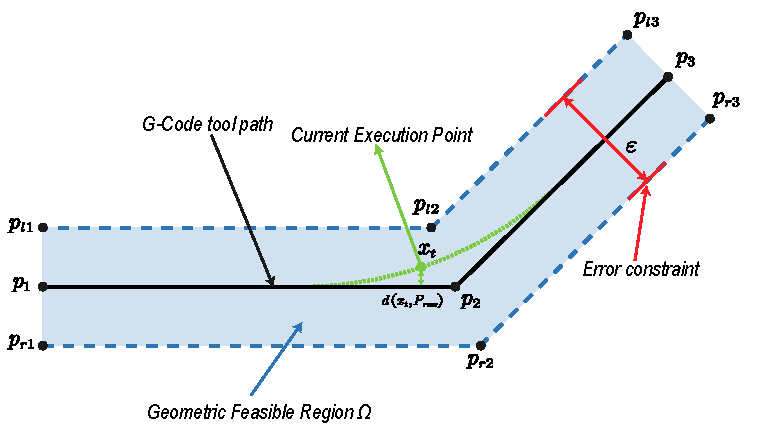
\includegraphics[width=0.9\linewidth]{Figure_2.pdf}
\caption{Geometric feasible region formed by the reference path and the contour tolerance band.}
\label{fig:feasible_region}
\end{figure}

For closed-loop decision making, the reference path is parameterized by arc length. At the current projected arc length $\ell_t$, local geometric quantities are extracted, including the normal error, tangential direction, distance to the next corner, and turning angle of the next corner. These quantities are used in the state representation, reward weighting, and corner-mode identification.

\subsection{Constrained Action Decision Formulation}
At each interpolation period $\Delta t$, the policy receives the current state $s_t$ and outputs a normalized action $a_t^{\pi}$. The kinematic constraint module (KCM) projects this action into an executable control command, which is then applied to the environment. The environment updates the position, orientation, and kinematic state, and returns the immediate reward $r_t$. The task is therefore written as a constrained sequential decision-making problem:
\begin{equation}
\max_{\pi}\ \mathbb{E}{\pi}\left[\sum{t=0}^{T} \gamma^t r_t\right],
\end{equation}
subject to the geometric constraint
\begin{equation}
x_t\in \Omega,
\end{equation}
and the execution-side kinematic constraints
\begin{equation}
|v_t|\leq V_{\max},\quad |a_t|\leq A_{\max},\quad |j_t|\leq J_{\max},
\end{equation}
\begin{equation}
|\omega_t|\leq \Omega_{\max},\quad |\dot{\omega}t|\leq A{\max}^{\omega},\quad |\ddot{\omega}t|\leq J{\max}^{\omega}.
\end{equation}
Here, $v_t$, $a_t$, and $j_t$ denote the linear velocity, linear acceleration, and linear jerk, respectively, whereas $\omega_t$, $\dot{\omega}_t$, and $\ddot{\omega}_t$ denote the angular velocity, angular acceleration, and angular jerk, respectively.

\section{Methodology}
\label{sec:methodology}
\subsection{Overall Framework}
Motion planning for hybrid tool paths is formulated as a closed-loop decision process in a reinforcement learning setting. The policy network acts as the agent, and the tool-path simulation system, which accounts for contour tolerance and kinematic constraints, acts as the environment. At each interpolation cycle, the environment builds the state $s_t$ from the current execution position, kinematic state, local corner information, and look-ahead geometry. Given $s_t$, the policy $\pi_\theta$ produces an action $a_t$ that gives the steering, feedrate, and look-ahead-distance adjustment commands for the current cycle. The action is corrected by the KCM and then applied to the environment. The environment moves to the next state $s_{t+1}$ and returns a reward $r_t$ based on path progress, contour error, and motion smoothness. During training, reward feedback updates the policy parameters, enabling the policy to learn a control law for trajectory smoothing, feedrate planning, and kinematic-constraint satisfaction within the tolerance band.

\figref{fig:framework} shows the overall framework of the proposed method. Given a reference path and a contour tolerance, the environment carries out path projection, corner scanning, and look-ahead geometry extraction to form a structured state vector at the current time step. The policy network outputs a normalized action. The steering and feedrate components are mapped to the pre-projection motion control variables $(\omega^{pre}_t, v^{pre}_t)$, and the look-ahead component is mapped to the current look-ahead distance $L_t$. The KCM then uses the velocity, acceleration, and jerk states from the previous time step to project $(\omega^{pre}_t, v^{pre}_t)$ onto the feasible kinematic set. This projection gives the executable control variables $(\omega_t, v_t)$, which satisfy the velocity, acceleration, and jerk limits. The execution result updates the current position, kinematic quantities, corner phase, and look-ahead observations. During training, the same result also enters the policy update through the reward signal. The whole procedure forms a closed reinforcement learning loop for motion planning.

\begin{figure}[htbp]
\centering
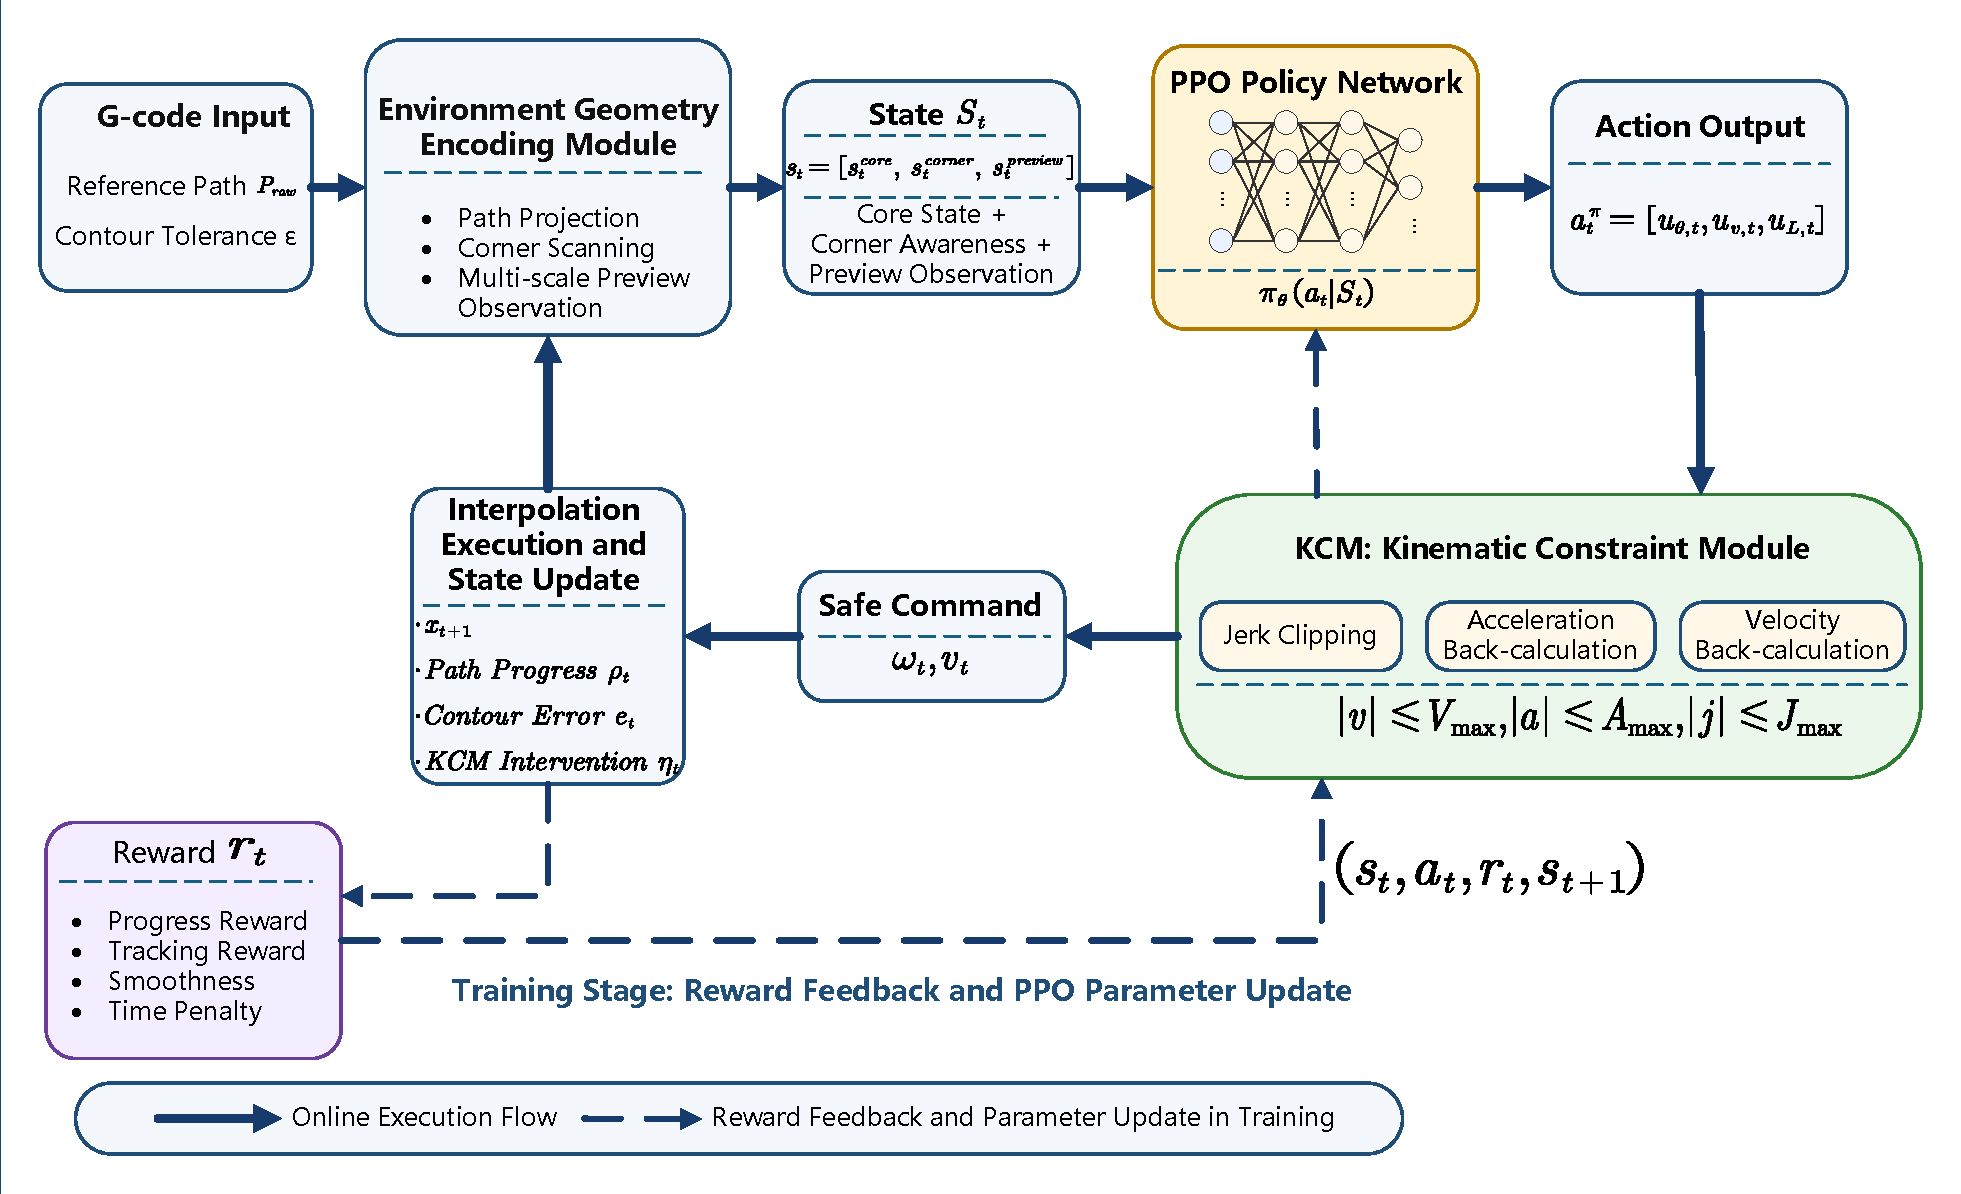
\includegraphics[width=0.9\linewidth]{Figure_3.pdf}
\caption{Overall closed-loop framework of the proposed method.}
\label{fig:framework}
\end{figure}

\subsection{State Design}
A hierarchical structured state representation is used:
\begin{equation}
s_t=[s_t^{core},\ s_t^{corner},\ s_t^{preview}].
\end{equation}
Here, $s_t^{core}$ describes the local tracking and kinematic state at the current time step, $s_t^{corner}$ describes the relation between the current path segment and the next corner, and $s_t^{preview}$ records the geometric trend over several preview distances ahead.

The core state is an eight-dimensional vector:
\begin{equation}
s_t^{core}=[\bar e_t,\ \bar e_{n,t},\ \bar\tau_t,\ \bar v_t,\ \bar a_t,\ \bar\omega_t,\ \rho_t,\ \bar d_{c,t}],
\end{equation}
where $\bar e_t$ is the normalized contour error, $\bar e_{n,t}$ is the signed normal error, and $\bar\tau_t$ is the normalized angular error between the current heading and the local tangent direction. The terms $\bar v_t$, $\bar a_t$, and $\bar\omega_t$ are the normalized linear velocity, linear acceleration, and angular velocity, respectively. In addition, $\rho_t\in[0,1]$ gives the overall path progress, and $\bar d_{c,t}$ is the normalized distance to the next corner.

The corner-aware state is a four-dimensional feature vector:
\begin{equation}
s_t^{corner}=[\bar\phi_t,\ \sigma_t,\ m_t,\ \sigma_t\bar e_{n,t}],
\end{equation}
where $\bar\phi_t$ is the normalized turning angle of the next corner, $\sigma_t\in{-1,0,1}$ is the turning sign of the corner, and $m_t\in{0,1}$ indicates whether the current position is within the corner-influence interval. The last term, $\sigma_t\bar e_{n,t}$, encodes the signed positional relation to the inner or outer side of the turn.

For preview observation, several preview scales ${\lambda_k}{k=1}^{N_L}$ are defined along the arc length of the reference path. Let $\ell_t$ be the arc-length coordinate of the projection of the current execution point onto the reference path. The forward observation point for the $k$-th preview scale is
\begin{equation}
q_t^{(k)}=P{\mathrm{raw}}(\ell_t+\lambda_k L_t),\qquad k=1,\dots,N_L,
\end{equation}
where $\lambda_k$ is the scale coefficient and $L_t$ is the base preview distance used in the current cycle. In this formulation, the near-, medium-, and far-range preview points are determined along the arc length of the reference path, rather than from ray intersections along the current execution direction. For each scale, the angular variation of the forward observation point relative to the current tangent direction and the corresponding distance ratio are extracted:
\begin{equation}
s_t^{preview}=\big[\Delta \theta_t^{(1)},\ \bar d_t^{(1)},\ \dots,\ \Delta \theta_t^{(N_L)},\ \bar d_t^{(N_L)}\big].
\end{equation}
Here, $\Delta \theta_t^{(k)}$ describes the directional change at the $k$-th preview scale, and $\bar d_t^{(k)}$ is the normalized distance from the current position to the corresponding preview point. The main implementation uses three preview scales.

\subsection{Action Space and Kinematic Constraint Module}
At each control cycle, the policy network outputs a normalized action:
\begin{equation}
a_t^{\pi}=[u_{\theta,t},u_{v,t},u_{L,t}],
\end{equation}
where $u_{\theta,t}\in[-1,1]$ is the normalized steering component, $u_{v,t}\in[0,1]$ is the normalized feedrate component, and $u_{L,t}\in[0,1]$ is the preview-distance adjustment component. Given the admissible preview-distance range $[L_{\min},L_{\max}]$, the physical preview distance is mapped as
\begin{equation}
L_t=L_{\min}+u_{L,t}(L_{\max}-L_{\min}).
\end{equation}
The policy output is first converted to pre-projection motion control variables in physical units:
\begin{equation}
\omega_t^{pre}=u_{\theta,t}\Omega_{\max},\qquad v_t^{pre}=u_{v,t}V_{\max}.
\end{equation}
The preview distance $L_t$ is used to compute the local reference direction and preview geometry. The KCM then projects $(\omega_t^{pre},v_t^{pre})$ onto the kinematically feasible set according to the kinematic state at the previous time step. For the linear-velocity channel, let $v_{t-1}$ and $a_{t-1}$ be the linear velocity and linear acceleration in the previous cycle. The pre-projection acceleration is
\begin{equation}
a_t^{pre}=\frac{v_t^{pre}-v_{t-1}}{\Delta t},
\end{equation}
and the corresponding pre-projection jerk is
\begin{equation}
j_t^{pre}=\frac{a_t^{pre}-a_{t-1}}{\Delta t}.
\end{equation}
The KCM clips this jerk by the jerk bound:
\begin{equation}
j_t=\mathrm{clip}(j_t^{pre},-J_{\max},J_{\max}),
\end{equation}
and then reconstructs the realizable acceleration and velocity for the current cycle:
\begin{equation}
a_t=\mathrm{clip}(a_{t-1}+j_t\Delta t,-A_{\max},A_{\max}),
\end{equation}
\begin{equation}
v_t=\mathrm{clip}\left(v_{t-1}+a_{t-1}\Delta t+\frac{1}{2}j_t\Delta t^2,0,V_{\max}\right).
\end{equation}
The angular-velocity channel uses the same projection procedure. The resulting $(\omega_t,v_t)$ is then applied to the environment as the executable control input. The resulting online projection procedure is summarized in Algorithm~\ref{alg:kcm_projection}.

\begin{algorithm}[H]
\caption{KCM-constrained action projection}
\label{alg:kcm_projection}
\begin{algorithmic}[1]
\Require Policy output $a_t^{\pi}=[u_{\theta,t},u_{v,t},u_{L,t}]$; previous-step kinematic state $(v_{t-1},a_{t-1},\omega_{t-1},\alpha_{t-1})$
\Ensure Executed control variables $(\omega_t,v_t)$ and the updated kinematic state
\State Map $u_{\theta,t}$ and $u_{v,t}$ to the unconstrained motion commands $(\omega_t^{pre},v_t^{pre})$
\State Map $u_{L,t}$ to the look-ahead distance $L_t$
\State Compute the unconstrained linear acceleration $a_t^{pre}$ from $v_t^{pre}$ and $v_{t-1}$
\State Compute the unconstrained linear jerk $j_t^{pre}$ from $a_t^{pre}$ and $a_{t-1}$
\State Clip $j_t^{pre}$ to obtain $j_t$ under the prescribed jerk bound
\State Recover the linear acceleration $a_t$ from $j_t$ and apply acceleration clipping
\State Integrate $(v_{t-1},a_{t-1},j_t)$ to obtain the linear velocity $v_t$ for the current control cycle
\State Apply the same procedure to the angular-velocity channel to obtain the constrained angular velocity $\omega_t$
\State Return the executed control variables $(\omega_t,v_t)$ and the updated kinematic state
\end{algorithmic}
\end{algorithm}

The intervention degree of the KCM is defined as
\begin{equation}
\eta_t=\frac{|v_t-v_t^{pre}|}{V_{\max}}+\frac{|\omega_t-\omega_t^{pre}|}{\Omega_{\max}}.
\end{equation}
This scalar is not part of the primary optimization objective. It is used only as an auxiliary metric in the result analysis.

\subsection{Reward Design}
The instantaneous reward is
\begin{equation}
r_t=r_t^{prog}+r_t^{track}+r_t^{dir}+r_t^{smooth}.
\label{eq:reward_total}
\end{equation}

The progress reward is defined as
\begin{equation}
r_t^{prog}=w_p\max(0,\rho_t-\rho_{t-1}),
\end{equation}
where $\rho_t$ is the overall path progress.

The contour-error penalty is defined as
\begin{equation}
\phi_e(e_t)=
\begin{cases}
0, & |e_{n,t}|\leq \delta_t,\\[4pt]
\left(\dfrac{|e_{n,t}|-\delta_t}{\varepsilon/2}\right)^2, & |e_{n,t}|>\delta_t,
\end{cases}
\end{equation}
and the corresponding tracking reward is
\begin{equation}
r_t^{track}=-w_e(c_t)\phi_e(e_t).
\end{equation}
Here, $\delta_t$ is the relaxed boundary within the tolerance band, and $c_t\in[0,1]$ is the local corner intensity. They are defined as
\begin{equation}
\delta_t=\kappa_{\delta}\frac{\varepsilon}{2}\mathbf{1}(m_t=1),
\end{equation}
\begin{equation}
c_t=\mathrm{clip}\left((1-\alpha_c)c_{t-1}+\alpha_c\frac{|\Delta\theta_t^{(N_L)}|}{\theta_0},0,1\right),
\end{equation}
where $\kappa_{\delta}$ is the error-relaxation ratio, $m_t$ indicates whether the current state is within the corner-influence region, $\Delta\theta_t^{(N_L)}$ is the look-ahead directional change at the farthest scale, $\theta_0$ is the normalization angle for local corner intensity, and $\alpha_c=1/T_c$ is the exponential moving-average coefficient. In the main experiments, $\kappa_{\delta}$ is set to $0$. Thus, the contour-error term has no additional dead zone, while $c_t$ is still used to adjust the tracking and smoothness weights.

The directional consistency term is defined as
\begin{equation}
r_t^{dir}=-w_{\tau}|\tau_t|,
\end{equation}
where $\tau_t$ is the angular error between the current heading and the local reference direction.

The smoothness term is defined as
\begin{equation}
r_t^{smooth}=-w_s(c_t)\psi_t,
\end{equation}
where $\psi_t$ can be a normalized measure of linear jerk, angular acceleration, or angular jerk. The weight $w_s(c_t)$ is adjusted according to the local corner intensity. One implementation is
\begin{equation}
w_s(c_t)=w_s^0 c_t^{\gamma}, \qquad \gamma>1,
\end{equation}
where $w_s(c_t)$ increases with $c_t$.

\subsection{PPO Training Configuration}
\label{sec:ppo_training_configuration}
The policy is trained with Proximal Policy Optimization (PPO). The Actor is a shared multilayer perceptron with three hidden layers of widths $256$, $128$, and $64$. Each layer uses ELU activation followed by LayerNorm. Separate output heads parameterize the mean and standard deviation of a three-dimensional action distribution. The steering mean is mapped to $[-1,1]$ with $\tanh$, while the feedrate and look-ahead means are mapped to $[0,1]$ with the sigmoid function. The standard deviation is obtained by applying the softplus function and then adding $10^{-3}$ for numerical stability. The Critic has layer widths $256,128,64,1$ and uses ELU activation, LayerNorm, and a dropout rate of $0.1$. The main training hyperparameters are listed in \tabref{tab:ppo_params}.

\begin{table}[H]
\centering
\caption{PPO hyperparameters and training protocol.}
\label{tab:ppo_params}
\small
\begin{tabular}{lp{0.68\textwidth}}
\toprule
\textbf{Parameter} & \textbf{Value}\\
\midrule
Actor learning rate & $3.0\times10^{-4}$\\
Critic learning rate & $1.5\times10^{-4}$\\
Discount factor $\gamma$ & $0.99$\\
GAE parameter $\lambda$ & $0.95$\\
PPO clip coefficient & $0.1$\\
Number of epochs per update & $8$\\
Entropy coefficient & $0.01$\\
Gradient clipping & $0.5$\\
\bottomrule
\end{tabular}
\end{table}

\section{Experiments and Results}
\label{sec:experiments_results}
This section evaluates the motion-planning performance of the proposed method on geometric paths with different characteristics through simulation experiments. The evaluation focuses on three aspects: whether the tool motion can advance stably along the reference path, whether the planned trajectory can generate reasonable transitions within the tolerance band, and whether the executed control variables satisfy the prescribed velocity, acceleration, and jerk constraints. The evaluation consists of a main comparative experiment and a set of ablation experiments. The main comparative experiment compares J-NNC with the neural network controller (NNC) baseline, whereas the ablation experiments separately modify the preview distance, KCM, preview observation, and reward scheduling to analyze the contribution of each module to the overall performance.

\subsection{Experimental Settings}

The experiments use three representative paths: a square path, a circular path, and a butterfly-shaped path. The circular path has continuous turning characteristics and is mainly used to examine the ability of the policy to maintain the feedrate and control the contour error under continuous-curvature conditions. The square path contains typical sharp corners and is used to evaluate the deceleration, turning, and re-acceleration behavior of the policy during corner entry, corner traversal, and corner exit. The butterfly-shaped path includes local curvature variations and geometric shape changes, and is used to assess the continuous path-following capability and trajectory control performance of the policy on complex geometric paths.

The main comparative experiment compares J-NNC with the NNC baseline. J-NNC adopts a structured state representation, a learnable look-ahead distance, KCM-based constraint enforcement, and a corner-aware reward. The NNC baseline is constructed following the direct neural control framework proposed by Li et al.~\cite{Li2020}, in which the policy output is directly applied to the environment for execution. The comparison between the two methods focuses on path advancement capability, contour error, and satisfaction of kinematic constraints.

The ablation experiments are constructed by modifying the proposed method. In the fixed-look-ahead configuration, the learnable look-ahead distance is replaced with a fixed look-ahead length. In the no-KCM configuration, the execution-layer kinematic-constraint projection is removed, so that the policy output is directly executed in the environment. In the no-look-ahead-observation configuration, the multi-scale forward geometric input is removed. In the no-straight/corner-dual-reward configuration, the differentiated reward scheduling for straight and corner segments is disabled. These configurations allow the effects of look-ahead distance, execution constraints, forward geometric information, and reward structure on the experimental results to be examined separately.

For evaluation, the reported trajectory exported from each configuration is used as the path-level evaluation sample instead of an average over multiple evaluation episodes. The metrics include the terminal state, final progress, maximum contour error, maximum relative violation of the linear-jerk limit, and termination time. The terminal state and final progress characterize path advancement, the maximum contour error measures the deviation of the trajectory from the reference path, and the maximum relative violation of the linear-jerk limit indicates whether the executed control commands satisfy the jerk constraint. The termination time is obtained by multiplying the terminal step of the reported trajectory by the interpolation period. Since this work studies constrained motion planning, the subsequent analysis jointly considers efficiency, error, and dynamic feasibility.

\subsection{Main Comparative Results}

This subsection reports the comparative results of J-NNC and the NNC baseline on three representative paths. \tabref{tab:main_results} summarizes the termination status, final progress, maximum contour error, maximum relative violation of the linear-jerk limit, and termination time for each method.


\begin{table}[H]
\centering
\caption{Comparison between J-NNC and the NNC baseline on representative evaluation trajectories.}
\label{tab:main_results}
\resizebox{0.92\textwidth}{!}{
\begin{tabular}{llcc}
\toprule
\textbf{Path} & \textbf{Metric} & \textbf{J-NNC} & \textbf{NNC baseline}\\
\midrule
\multirow{5}{*}{square} & Termination status & success & success\\
& Final progress & 1.000 & 1.000\\
& Maximum contour error & 0.834 & 0.676\\
& Maximum relative linear-jerk exceedance & 0.000 & 3199.000\\
& Termination time (s) & 12.192 & 8.672\\
\midrule
\multirow{5}{*}{circle} & Termination status & success & max\_steps\\
& Final progress & 1.000 & 0.990\\
& Maximum contour error & 0.096 & 6.259\\
& Maximum relative linear-jerk exceedance & 0.000 & 3199.000\\
& Termination time (s) & 9.117 & 60.000\\
\midrule
\multirow{5}{*}{butterfly} & Termination status & success & success\\
& Final progress & 1.000 & 1.000\\
& Maximum contour error & 0.745 & 0.207\\
& Maximum relative linear-jerk exceedance & 0.000 & 3199.000\\
& Termination time (s) & 10.480 & 5.807\\
\bottomrule
\end{tabular}
}
\end{table}



\tabref{tab:main_results} shows that J-NNC achieves successful termination on the square, circular, and butterfly-shaped paths. The NNC baseline also terminates successfully on the square and butterfly-shaped paths, whereas it reaches the maximum step limit on the circular path. A further comparison indicates that the main advantage of J-NNC lies in its ability to satisfy the kinematic constraints. For all three paths, J-NNC keeps the maximum relative violation of linear jerk at zero. The NNC baseline demonstrates path-advancement capability, but without an explicit execution-layer projection, its raw actions may violate jerk limits under the tested constraints. After KCM is introduced, the policy outputs are converted into executable control commands that satisfy the velocity, acceleration, and jerk limits.

From the perspective of path geometry, the circular path mainly evaluates control performance under continuous turning. The results for the circular path in \tabref{tab:main_results} show that J-NNC terminates successfully and keeps both the contour error and the jerk constraint within acceptable ranges. The NNC baseline reaches the maximum step limit on this path. The square path contains sharp corners and a closed endpoint. Both methods complete this path, and their differences mainly appear in trajectory handling near the corners and in jerk-constraint satisfaction. The trajectory generated by the NNC baseline is closer to the original polyline, with more concentrated direction changes. J-NNC forms local transitions within the tolerance band and limits the executed control commands through KCM. The butterfly-shaped path involves more complex curvature variations. The NNC baseline may show numerical advantages in some efficiency or error metrics, yet the absence of explicit jerk-constrained projection limits its dynamic executability under the prescribed machine-tool constraints. In contrast, J-NNC satisfies the kinematic constraints through a more conservative execution process.

\figref{fig:qualitative_results} presents the trajectory comparisons on the three paths.


\begin{figure}[!htbp]
\centering
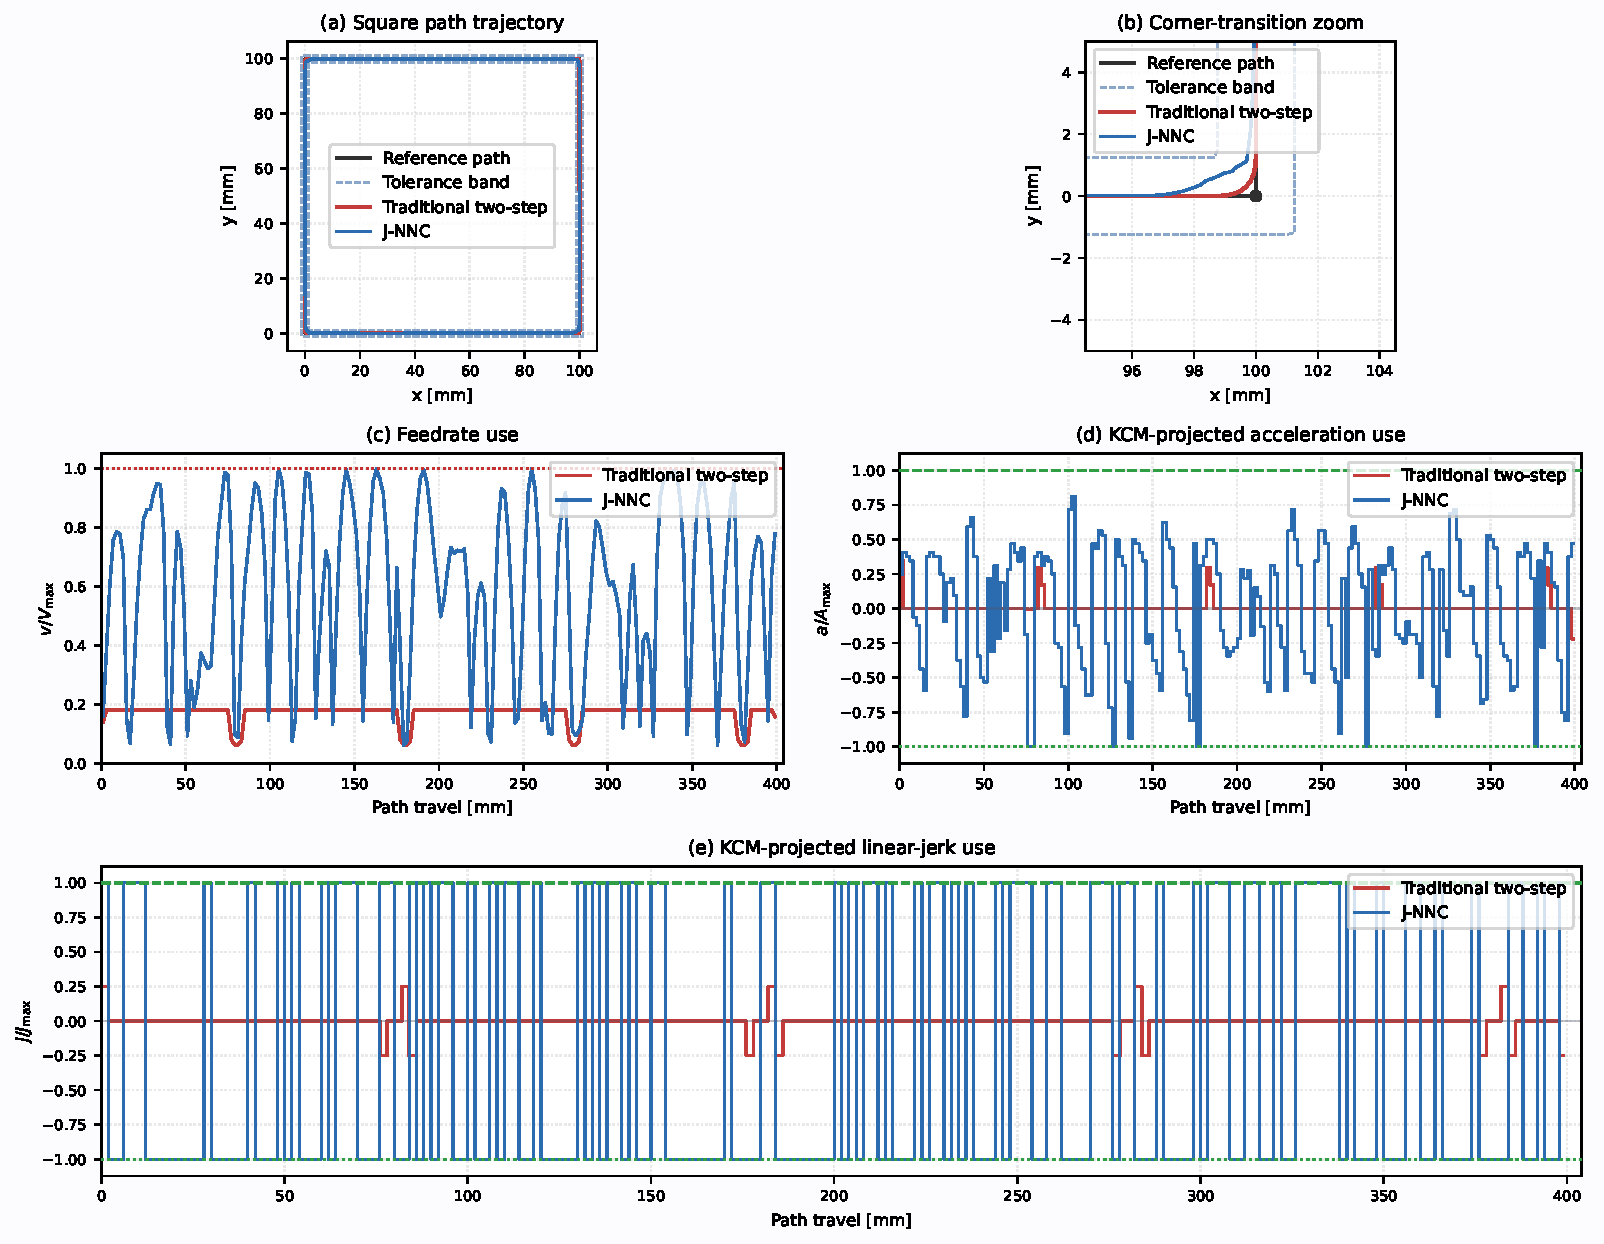
\includegraphics[width=0.96\linewidth]{Figure_4.pdf}
\caption{Trajectory comparison between J-NNC and the NNC baseline on representative paths: (a) square path, J-NNC; (b) square path, NNC baseline; (c) circular path, J-NNC; (d) circular path, NNC baseline; (e) butterfly-shaped path, J-NNC; (f) butterfly-shaped path, NNC baseline.}
\label{fig:qualitative_results}
\end{figure}


In \figref{fig:qualitative_results}(a)--(f), the trajectories generated by J-NNC remain within the tolerance band and do not exactly coincide with the reference polyline. On the square path, \figref{fig:qualitative_results}(a) shows that J-NNC forms local corner transitions, whereas \figref{fig:qualitative_results}(b) shows that the NNC baseline follows the original polyline more closely. On the circular path, \figref{fig:qualitative_results}(c) shows continuous advancement with relatively smooth velocity variation, while \figref{fig:qualitative_results}(d) reflects the baseline behavior under continuous turning. On the butterfly-shaped path, \figref{fig:qualitative_results}(e) shows moderate offsets in curvature-changing regions, while \figref{fig:qualitative_results}(f) provides the corresponding NNC baseline. These observations indicate that J-NNC uses the tolerance band to adjust the local trajectory, thereby reducing abrupt control changes near corners or varying-curvature regions.

The corner region of the square path is compared in \figref{fig:square_corner_zoom}.


\begin{figure}[!htbp]
\centering
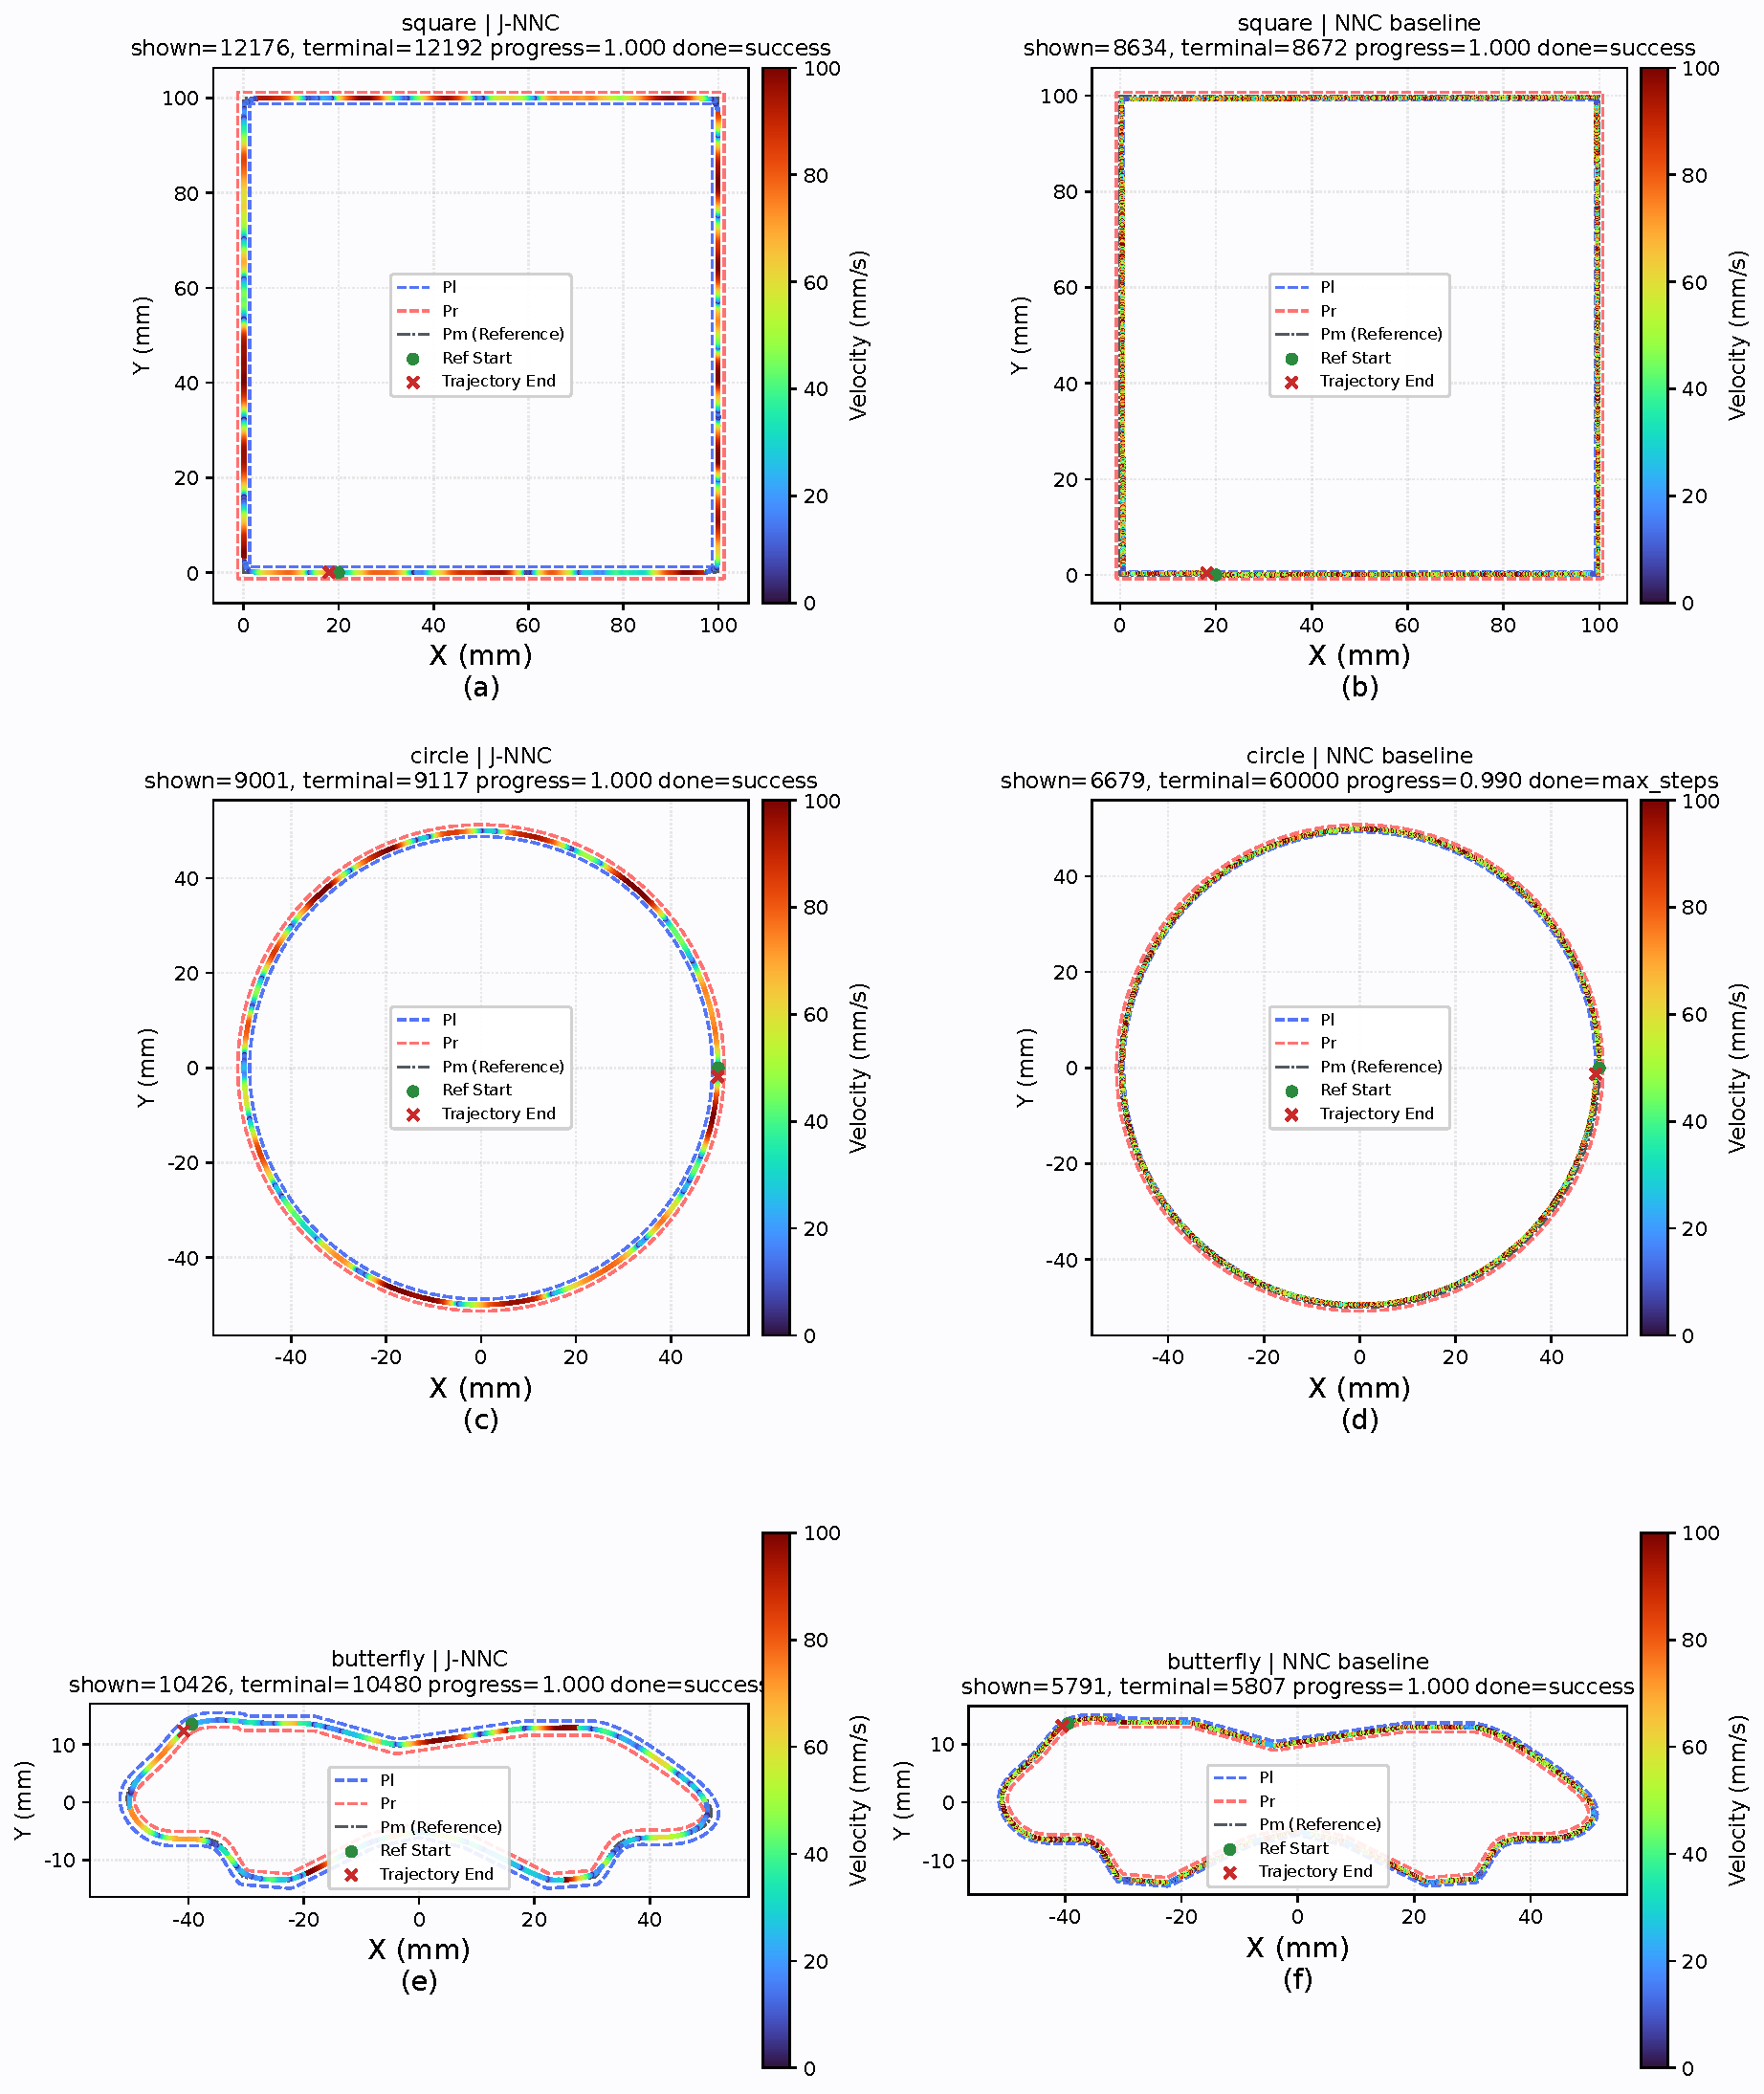
\includegraphics[width=0.82\linewidth]{Figure_5.pdf}
\caption{Local zoomed-in comparison in the square-corner region: (a) J-NNC; (b) NNC baseline.}
\label{fig:square_corner_zoom}
\end{figure}


\figref{fig:square_corner_zoom}(a) shows that J-NNC begins to change the motion direction before approaching the corner and forms a continuous transition trajectory within the tolerance band. In contrast, \figref{fig:square_corner_zoom}(b) shows that the NNC baseline remains closer to the original polyline, with the direction change concentrated near the corner point. This observation is consistent with the jerk results reported in \tabref{tab:main_results}. When the policy outputs are executed directly, large dynamic variations tend to occur at the corners. After the KCM constraint is applied, J-NNC satisfies the jerk limit during turning.

The normalized time histories of contour error, velocity, and linear jerk for J-NNC on a representative evaluation trajectory are shown in \figref{fig:kcm_analysis}.


\begin{figure}[!htbp]
\centering
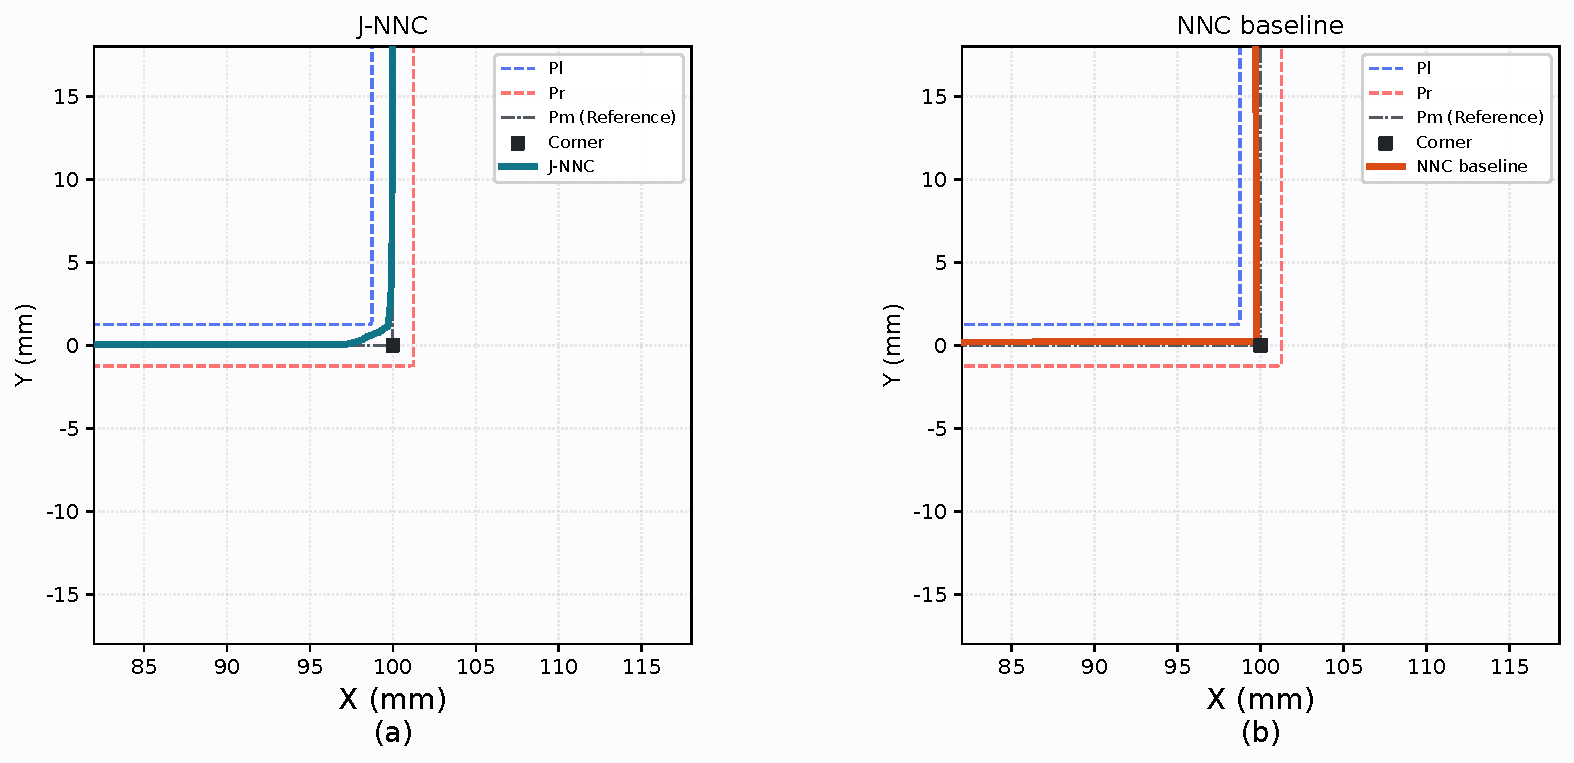
\includegraphics[width=0.9\linewidth]{Figure_6.pdf}
\caption{Representative evaluation behavior of J-NNC: (a) contour error; (b) velocity; (c) normalized linear jerk.}
\label{fig:kcm_analysis}
\end{figure}


In \figref{fig:kcm_analysis}(a), the peak contour errors mainly occur during cornering, indicating that the policy uses the available spatial margin within the tolerance band. \figref{fig:kcm_analysis}(b) reflects the speed modulation process during corner entry, corner traversal, and corner exit. \figref{fig:kcm_analysis}(c) reports the windowed peak $|j|/J_{\max}$ curve obtained by rechecking the velocity records of the same reported trajectory against the KCM boundary. This curve remains no greater than 1. Together with \tabref{tab:main_results}, this result shows that the maximum relative exceedance of linear jerk is zero after KCM is enabled.

\Needspace{12\baselineskip}

The combined results in \tabref{tab:main_results} and \figref{fig:qualitative_results}--\figref{fig:kcm_analysis} show that J-NNC completes the reported evaluation trajectory on all three types of paths and forms locally smooth trajectories within the tolerance band in both high-speed linear feeding segments and corner regions. For the sharp corners of the square path and the mixed-curvature regions of the butterfly-shaped path, J-NNC keeps the executed control quantities within the kinematic boundaries at corners or curvature-transition regions through appropriate trajectory smoothing and KCM constraints. The NNC baseline demonstrates path-advancement capability, while the absence of explicit constraint handling limits its dynamic feasibility.

\subsection{Ablation Results}

The ablation study removes or modifies the learnable look-ahead distance, KCM, look-ahead observation, and dual straight-line/corner reward modules. \tabref{tab:ablation} reports, for the reported evaluation trajectory on each path, the termination status, final progress, maximum contour error, maximum relative violation of the linear jerk limit, and termination time under each configuration.


\begin{table}[H]
\centering
\caption{Path-level reported evaluation results of the structured ablation study.}
\label{tab:ablation}
\resizebox{0.98\textwidth}{!}{
\begin{tabular}{llccccc}
\toprule
\textbf{Model configuration} & \textbf{Path} & \textbf{Termination status} & \textbf{Final progress} & \textbf{Maximum contour error} & \textbf{Maximum relative linear-jerk violation} & \textbf{Termination time (s)}\\
\midrule
J-NNC & square & success & 1.000 & 0.834 & 0.000 & 12.192\\
J-NNC & circle & success & 1.000 & 0.096 & 0.000 & 9.117\\
J-NNC & butterfly & success & 1.000 & 0.745 & 0.000 & 10.480\\
\midrule
Fixed look-ahead & square & success & 1.000 & 0.699 & 0.000 & 8.680\\
Fixed look-ahead & circle & success & 1.000 & 0.046 & 0.000 & 4.804\\
Fixed look-ahead & butterfly & success & 1.000 & 0.638 & 0.000 & 5.049\\
\midrule
Without KCM & square & success & 1.000 & 0.722 & 3199.000 & 10.301\\
Without KCM & circle & success & 1.000 & 0.061 & 3199.000 & 5.926\\
Without KCM & butterfly & success & 1.000 & 0.707 & 3199.000 & 7.446\\
\midrule
Without look-ahead observation & square & success & 1.000 & 0.805 & 0.000 & 8.151\\
Without look-ahead observation & circle & success & 1.000 & 0.077 & 0.000 & 4.573\\
Without look-ahead observation & butterfly & success & 1.000 & 0.820 & 0.000 & 6.044\\
\midrule
Without straight-line/corner dual rewards & square & success & 1.000 & 0.824 & 0.000 & 15.132\\
Without straight-line/corner dual rewards & circle & success & 1.000 & 0.030 & 0.000 & 10.388\\
Without straight-line/corner dual rewards & butterfly & success & 1.000 & 0.918 & 0.000 & 9.623\\
\bottomrule
\end{tabular}
}
\end{table}



\tabref{tab:ablation} shows that all ablated configurations terminate successfully in the reported evaluation runs on the three paths, although they differ in termination time, contour error, and jerk constraint satisfaction. The fixed look-ahead setting isolates the effect of online look-ahead distance adjustment. Removing look-ahead observation tests the contribution of multi-scale geometric information, while removing the dual straight-line/corner reward tests the effect of phase-dependent reward weights. The setting without KCM is used to examine the role of constraint projection at the execution layer. Since KCM is enabled in all other settings, the maximum relative violation of the linear jerk limit is zero for those settings.

\figref{fig:jerk_constraint_comparison} compares the linear jerk of J-NNC with that of the setting without KCM on the same representative path.


\begin{figure}[htbp]
\centering
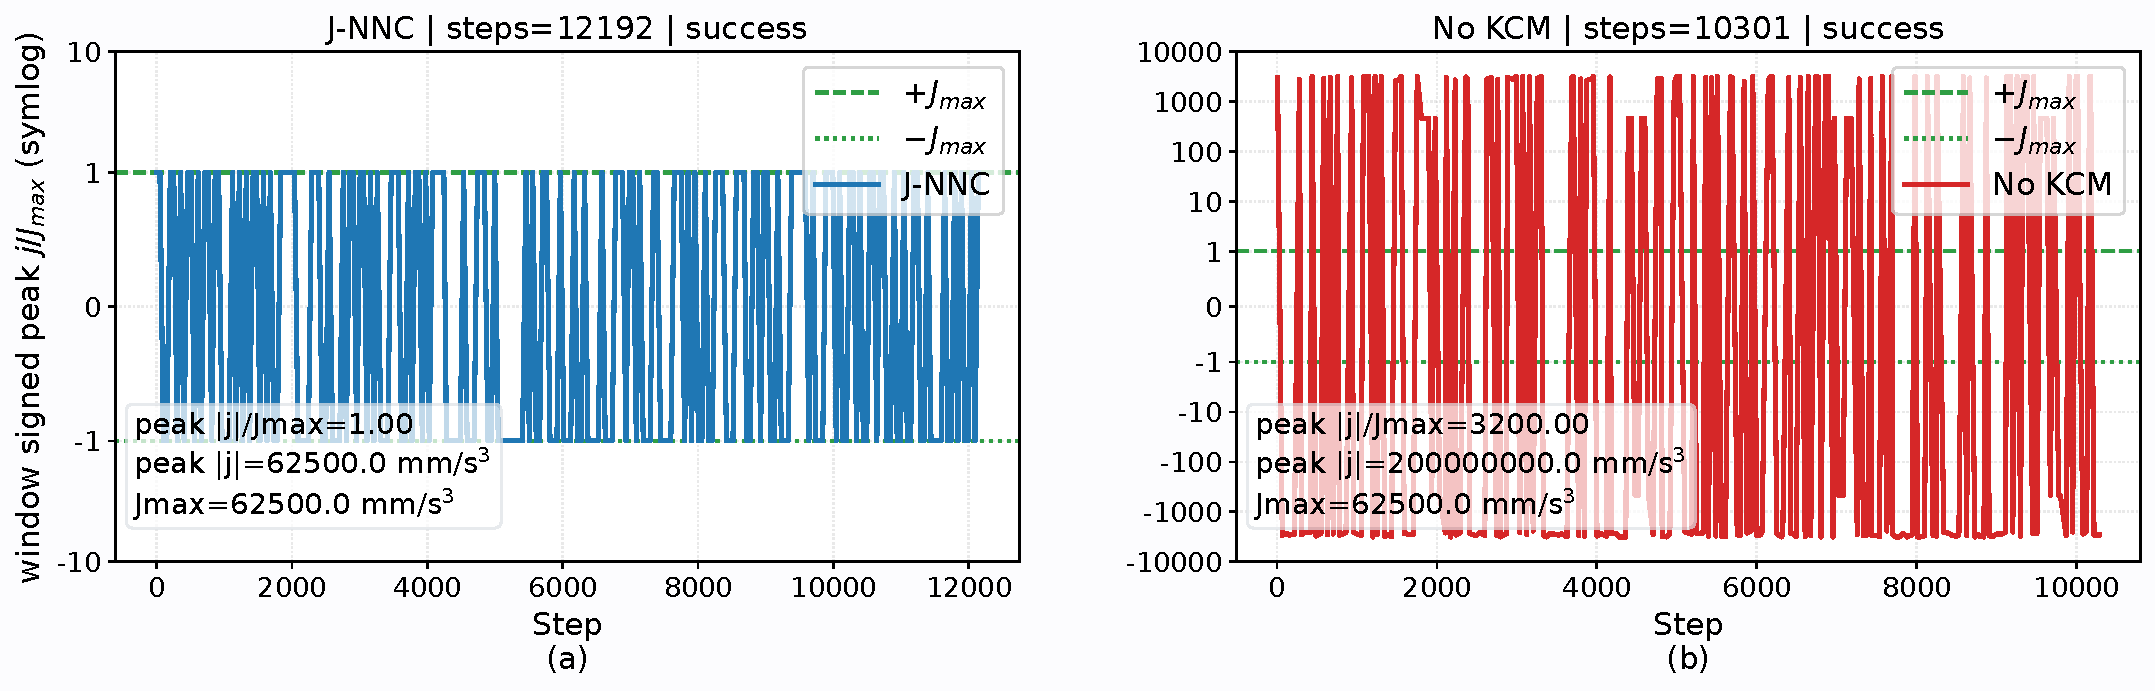
\includegraphics[width=0.96\linewidth]{Figure_7.pdf}
\caption{Linear-jerk constraint comparison on the same representative path: (a) J-NNC with KCM; (b) ablated configuration without KCM.}
\label{fig:jerk_constraint_comparison}
\end{figure}


As shown in \figref{fig:jerk_constraint_comparison}(a), the linear jerk of J-NNC stays within the bound defined by $J_{\max}$. By contrast, \figref{fig:jerk_constraint_comparison}(b) shows high-amplitude jerk spikes after KCM is removed. This result suggests that shorter execution time or smaller contour error alone is not sufficient to guarantee an executable trajectory. KCM is therefore a necessary part of the proposed method because it maps policy outputs to executable control commands that satisfy velocity, acceleration, and jerk constraints.

The fixed look-ahead setting examines the role of look-ahead distance adjustment. It retains the forward geometric perception structure but uses a fixed look-ahead length for decision making. As shown in \tabref{tab:ablation}, this setting terminates successfully on all three paths, and it produces shorter termination times on some paths. The learnable look-ahead distance allows the policy to adjust the perception scale online, while also increasing the dimensionality of the action space. Its effect depends on path complexity, reward weights, and the degree of KCM intervention. The current results suggest that the parameterization of the look-ahead distance action still needs refinement, so that it can support anticipatory speed regulation and corner preprocessing more consistently. For this reason, its role should be assessed with metrics beyond termination time alone.

The setting without look-ahead observation examines the role of multi-scale forward geometric information. It retains the learnable look-ahead distance and KCM-constrained execution, but removes the multi-scale look-ahead observation state. As shown in \tabref{tab:ablation}, the local state and corner awareness are sufficient for basic progression on all three paths, with path-dependent changes in termination time and contour error. Multi-scale look-ahead observations give the policy more information about the upcoming geometric trend. This information is mainly useful for anticipatory deceleration, early steering, and velocity transition on complex hybrid paths. The benefit of this module should be further tested on longer paths, denser corner distributions, and more complex curvature profiles.

The setting without the straight-line/corner dual-reward scheme examines the role of phase-dependent reward design. It applies the same reward weights to straight-line feeding, corner entry, corner traversal, and corner exit. As shown in \tabref{tab:ablation}, removing this module reduces completion stability across paths. Straight segments mainly require stable feed motion and directional consistency, whereas corner segments require error regulation, limited velocity variation, and smooth steering. When the same reward weights are used for all phases, the policy is more prone to unstable behavior during transitions between straight segments and corner regions. The straight-line/corner dual-reward scheme therefore helps the policy learn control behaviors that depend on the local path geometry.

The results in \tabref{tab:ablation} and \figref{fig:jerk_constraint_comparison} indicate that KCM mainly ensures the dynamic feasibility of the executed trajectory, while the straight-line/corner dual-reward scheme mainly improves behavioral stability across geometric phases. The learnable look-ahead distance and multi-scale look-ahead observations provide forward geometric perception and online adjustment capability. The current results also show that, although the square closed path can be completed successfully, termination time and velocity continuity after corner traversal remain important factors for experimental efficiency and should be addressed in subsequent optimization.

\section{Conclusion}
\label{sec:conclusion}

This paper presented J-NNC, a reinforcement learning-based CNC motion-planning method for mixed CAM-generated tool paths subject to contour-tolerance and kinematic constraints. The main difficulty considered in this work is that geometric smoothing, feedrate planning, and dynamic feasibility cannot be treated independently in practical CNC interpolation. A trajectory that stays close to the reference polyline may still contain sharp direction changes near corners, while a learned controller that advances the path efficiently may produce commands that exceed velocity, acceleration, or jerk limits. J-NNC addresses this issue by treating CNC interpolation as a closed-loop constrained decision-making process, rather than as a serial procedure with separate smoothing and feedrate-planning stages. The structured state and learnable preview action allow the policy to combine tracking, kinematic, corner, and forward-geometric information when planning local transitions within the tolerance band. The KCM further projects learned steering and feedrate outputs into executable commands satisfying velocity, acceleration, and jerk limits. Experiments on square, circular, and butterfly-shaped paths show full path progress and zero maximum relative linear-jerk violation, confirming the importance of explicit action projection compared with the NNC baseline and the no-KCM ablation.

Future work will refine the preview-distance action and corner-phase representation to improve traversal efficiency and velocity continuity after corner transitions. Further validation will include servo lag, axis-level constraints, and real machining experiments to assess practical deployment on CNC systems.

\clearpage
\bibliographystyle{unsrt}
\bibliography{references}

\end{document}
